\documentclass[12pt]{article}

% ============================================================
% PACKAGES
% ============================================================
\usepackage[utf8]{inputenc}
\usepackage[T1]{fontenc}
\usepackage[
  margin=1.15in,
  top=1.15in,
  bottom=1.15in,
  left=1.35in,
  right=1.15in
]{geometry}

\usepackage{amsmath,amssymb,mathtools,bm}
\usepackage{enumitem}
\usepackage{xcolor,pagecolor,booktabs,array,microtype}
\usepackage[colorlinks=true,linkcolor=cyan,urlcolor=cyan,citecolor=green]{hyperref}
\usepackage[most]{tcolorbox}
\tcbuselibrary{breakable,skins}
\usepackage{tikz}
\usetikzlibrary{arrows.meta,calc,positioning,intersections,patterns,lindenmayersystems}
\usepackage[american]{circuitikz}
\usepackage{sectsty}
\usepackage{pgfornament}
\usepackage{lettrine}
\usepackage{ebgaramond}
\usepackage[pages=all]{background}
\usepackage{graphicx}
\usepackage{float}

\allowdisplaybreaks

% ============================================================
% NATURE DARK MODE COLORS
% ============================================================
\definecolor{BG}{HTML}{0D1410}
\definecolor{FG}{HTML}{E5EFE7}
\definecolor{PANEL}{HTML}{131D16}
\definecolor{PANEL2}{HTML}{19261E}
\definecolor{PANEL3}{HTML}{203025}

\definecolor{BLUE}{HTML}{48A9A6}
\definecolor{GREEN}{HTML}{73D055}
\definecolor{GOLD}{HTML}{D4A373}
\definecolor{RED}{HTML}{E76F51}
\definecolor{GRAY}{HTML}{8BA38B}
\definecolor{TEAL}{HTML}{2A9D8F}
\definecolor{PURPLE}{HTML}{B584D4}

\definecolor{FOREST}{HTML}{2D4233}
\definecolor{MOSS}{HTML}{3E5C43}
\definecolor{SEPIA}{HTML}{5F4B32}
\definecolor{LEAF}{HTML}{73D055}
\definecolor{BARK}{HTML}{8A6A43}

\pagecolor{BG}
\color{FG}

% ============================================================
% BACKGROUND WATERMARK
% ============================================================
\backgroundsetup{
  scale=3,
  color=GREEN,
  opacity=0.035,
  angle=0,
  contents={\pgfornament[width=12cm]{85}}
}

% ============================================================
% GLOBAL FORMATTING
% ============================================================
\setlength{\parindent}{0pt}
\setlength{\parskip}{0.45em}
\setlength{\emergencystretch}{4em}
\sloppy
\renewcommand{\arraystretch}{1.2}

\sectionfont{\color{BLUE}}
\subsectionfont{\color{GREEN}}
\subsubsectionfont{\color{GOLD}}

% ============================================================
% SECTION HEADER STYLE
% ============================================================
\newcommand{\sectionheader}[1]{%
  \vspace{0.7cm}
  \noindent{\Large\bfseries\color{BLUE}#1}
  \hfill
  \raisebox{-0.3em}{\textcolor{GREEN}{\pgfornament[width=1.8cm]{17}}}\par
  \vspace{0.15cm}
  \noindent\textcolor{BLUE}{\rule{\textwidth}{1.1pt}}
  \vspace{0.5cm}
}

% ============================================================
% COMMANDS
% ============================================================
\newcommand{\ds}{\displaystyle}
\newcommand{\Om}{\Omega}
\newcommand{\jj}{\mathrm{j}}
\newcommand{\ee}{\mathrm{e}}
\newcommand{\matlab}{\textsc{MATLAB}}
\newcommand{\simulink}{\textsc{Simulink}}

% ============================================================
% BOX STYLES
% ============================================================
\tcbset{
  enhanced,
  breakable,
  sharp corners,
  arc=0pt,
  outer arc=0pt,
  boxrule=0pt,
  frame hidden,
  colback=PANEL,
  coltext=FG,
  left=12pt,
  right=12pt,
  top=10pt,
  bottom=10pt,
  boxsep=6pt
}

\newtcolorbox{problem}[2][]{%
  borderline west={2.6pt}{0pt}{BLUE},
  colback=PANEL,
  overlay={
    \node[anchor=south east,font=\bfseries\Large,text=BLUE,inner sep=1pt]
    at ([xshift=-6pt,yshift=-6pt]frame.north west) (Pword) {Problem};
    \node[anchor=north east,fill=BLUE,text=BG,font=\bfseries,inner sep=3.2pt,
    minimum width=1.15cm,sharp corners] at ([yshift=-1pt]Pword.south east) {#2};
  },
  #1
}

\newtcolorbox{solution}[2][]{%
  borderline west={2.6pt}{0pt}{GREEN},
  colback=PANEL,
  overlay={
    \node[anchor=south east,font=\bfseries\Large,text=GREEN,inner sep=1pt]
    at ([xshift=-6pt,yshift=-6pt]frame.north west) (Sword) {Solution};
    \node[anchor=north east,fill=GREEN,text=BG,font=\bfseries,inner sep=3.2pt,
    minimum width=1.15cm,sharp corners] at ([yshift=-1pt]Sword.south east) {#2};
  },
  #1
}

\newtcolorbox{noteBox}[1][]{%
  borderline west={2.0pt}{0pt}{PURPLE},
  colback=PANEL2,
  coltext=FG,
  sharp corners,
  #1
}

% ============================================================
% BORDERLESS FIGURE MACRO
% This removes the surrounding tcolorbox and trims the baked-in white PNG margin.
% If white still shows, increase trim to 70 70 70 70.
% If too much is cut off, reduce trim to 35 35 35 35.
% ============================================================
\newcommand{\figmaybe}[3]{%
\IfFileExists{#1}{%
\begin{center}
\includegraphics[
  width=#2\linewidth,
  trim=55 55 55 55,
  clip
]{#1}

\vspace{2pt}
{\small\color{GRAY}#3}
\end{center}
}{%
\begin{noteBox}
\textbf{Missing figure.} Expected image:
\[
\texttt{\detokenize{#1}}
\]
Make sure the PNG exists in the project-level \texttt{\detokenize{figures/}} folder.
\end{noteBox}
}%
}

% ============================================================
% CIRCUITIKZ STYLE
% ============================================================
\ctikzset{
  bipoles/thickness=1.2,
  bipoles/length=1.1cm,
  inductors/coils=5,
  capacitors/scale=0.95,
  resistors/scale=0.95
}

% ============================================================
% DOCUMENT
% ============================================================
\begin{document}

\begin{center}
  \vspace*{0.35cm}

  \textcolor{GREEN}{\pgfornament[width=7cm]{88}}\\[1.5em]

  {\Huge\textit{\color{FG}ENEE 323}}\\[4pt]
  {\LARGE\textbf{\color{BLUE}Signal and System Theory}}\\[5pt]
  {\Large\color{GREEN}Project 6: Pulse Wave Response of a Passive Analog Filter}\\[8pt]

  {\color{GOLD}Third-Order Butterworth Lowpass RLC Filter: Theory, Fourier Series, IFFT, and Simulation}\\[6pt]
  {\color{FG}Yahya Mouamil}\\[2pt]
  {\color{FG}UID: 119873526}\\[2pt]
  {\color{FG}Date: May 2026}\\[1.5em]

  \textcolor{GREEN}{\pgfornament[width=7cm]{88}}
\end{center}

\vspace{0.7cm}

\lettrine[lines=3,lhang=0.18,nindent=0pt]
{\color{GREEN}T}{his} report studies the response of a third-order Butterworth lowpass filter to a periodic rectangular pulse train with period \(T_0=1\) s and duty cycle \(\alpha=40\%\). The work includes the frequency response, the output Fourier series, an IFFT reconstruction, and a time-domain comparison plot.

% ============================================================
\sectionheader{Setup: Circuit and Transfer Function}

\begin{noteBox}
The passive filter consists of two inductors, one shunt capacitor, and one load resistor. The input is \(x(t)\), and the output \(y(t)\) is the voltage across the \(100\,\Omega\) resistor.
\end{noteBox}

\begin{center}
\begin{tcolorbox}[
  enhanced,
  sharp corners,
  colback=PANEL2,
  colframe=PANEL2,
  boxrule=0pt,
  left=10pt,
  right=10pt,
  top=10pt,
  bottom=8pt,
  width=0.92\linewidth
]
\centering

\begin{circuitikz}[american voltages, line width=1.05pt, scale=1.08, transform shape]

    % Bottom wire
    \draw[FG] (0,0) -- (6.2,0);

    % Manual inverted voltage source:
    % minus on top, plus on bottom
    \draw[BLUE] (0,0) -- (0,1.05);
    \draw[BLUE] (0,1.95) -- (0,3.0);
    \draw[BLUE, fill=BG] (0,1.5) circle (0.45);
    \node[text=FG] at (0,1.72) {$-$};
    \node[text=FG] at (0,1.28) {$+$};
    \node[text=BLUE] at (-0.62,1.52) {$x(t)$};

    % Top wire and inductors
    \draw[FG] (0,3) -- (0.55,3);
    \draw[TEAL] (0.55,3) to[L, l=$9\,\mathrm{H}$] (3.0,3);
    \draw[GREEN] (3.0,3) to[L, l=$3\,\mathrm{H}$] (5.4,3);
    \draw[FG] (5.4,3) -- (6.2,3);

    % Capacitor branch
    \draw[GOLD] (3.0,3) to[C, l_=$800\,\mu\mathrm{F}$] (3.0,0);

    % Resistor branch
    \draw[RED] (6.2,3) to[R, l_=$100\,\Omega$, *-*] (6.2,0);

    % Ground
    \draw[GRAY] (3.0,0) node[sground] {};

    % Output labels
    \node[text=FG] at (6.62,3.0) {$+$};
    \node[text=BLUE] at (6.93,1.5) {$y(t)$};
    \node[text=FG] at (6.62,0.0) {$-$};

    % Connection dots
    \fill[FG] (3.0,3.0) circle (1.3pt);
    \fill[FG] (6.2,3.0) circle (1.3pt);
    \fill[FG] (6.2,0.0) circle (1.3pt);

\end{circuitikz}

\vspace{4pt}
{\small\color{GRAY}Third-order Butterworth lowpass RLC network.}
\end{tcolorbox}
\end{center}

The transfer function is
\[
H(s)
=
\frac{Y(s)}{X(s)}
=
\frac{1}{(s/\beta)^3+2(s/\beta)^2+2(s/\beta)+1},
\qquad
\beta=\frac{50}{3}\ \text{rad/s}.
\]

Multiplying numerator and denominator by \(\beta^3\), we may also write
\[
H(s)=\frac{\beta^3}{s^3+2\beta s^2+2\beta^2s+\beta^3}.
\]

Thus for MATLAB one convenient representation is
\[
\texttt{num}=\beta^3,
\qquad
\texttt{den}=
\begin{bmatrix}
1 & 2\beta & 2\beta^2 & \beta^3
\end{bmatrix}.
\]

The pulse-train parameters are
\[
T_0=1.0\ \text{s},
\qquad
\alpha=0.40,
\qquad
\Omega_0=\frac{2\pi}{T_0}=2\pi\ \text{rad/s}.
\]

% ============================================================
\sectionheader{Problem (i): Frequency Response}

\begin{problem}{i}
Using \texttt{polyval}, evaluate the complex frequency response \(H(\jj\Omega)\) for
\[
\Omega=0:(0.1)\Omega_0:(100)\Omega_0.
\]
Plot the magnitude response \(|H(\jj\Omega)|\) in dB and phase response \(\angle H(\jj\Omega)\). Confirm that
\[
\Omega=\beta=\frac{50}{3}\ \text{rad/s}
\]
is the \(-3\) dB point.
\end{problem}

\begin{solution}{i}
Substitute \(s=\jj\Omega\) into the transfer function:
\[
H(\jj\Omega)
=
\frac{1}{(\jj\Omega/\beta)^3+2(\jj\Omega/\beta)^2+2(\jj\Omega/\beta)+1}.
\]

At \(\Omega=\beta\),
\[
H(\jj\beta)=\frac{1}{\jj^3+2\jj^2+2\jj+1}.
\]
Using
\[
\jj^2=-1,
\qquad
\jj^3=-\jj,
\]
the denominator becomes
\[
-\jj-2+2\jj+1=-1+\jj.
\]
Hence
\[
H(\jj\beta)=\frac{1}{-1+\jj},
\]
so
\[
|H(\jj\beta)|=\frac{1}{\sqrt{(-1)^2+1^2}}=\frac{1}{\sqrt{2}}.
\]
Therefore
\[
20\log_{10}|H(\jj\beta)|
=
20\log_{10}\!\left(\frac{1}{\sqrt{2}}\right)
=
-3.0103\ \text{dB}.
\]

Thus
\[
\boxed{
\Omega=\beta=\frac{50}{3}\ \text{rad/s}
}
\]
is indeed the cutoff frequency.

\figmaybe{../figures/part_i_frequency_response.png}{0.99}{Part (i): magnitude and phase response of the Butterworth lowpass filter.}
\end{solution}

% ============================================================
\sectionheader{Problem (ii): Output Fourier Series}

\begin{problem}{ii}
The input pulse train has complex Fourier series
\[
x(t)=\sum_{k=-\infty}^{\infty} X_k \ee^{\jj k\Omega_0 t},
\qquad
X_k=\frac{\sin(k\alpha\pi)}{k\pi},
\]
with \(X_0=\alpha\). Write the complex Fourier series of the output \(y(t)\), and then express it as a cosine sum over nonnegative harmonic indices.
\end{problem}

\begin{solution}{ii}
Because the system is linear and time-invariant,
\[
Y_k=X_kH(\jj k\Omega_0).
\]
Therefore,
\[
\boxed{
y(t)
=
\sum_{k=-\infty}^{\infty}
X_kH(\jj k\Omega_0)\ee^{\jj k\Omega_0t}.
}
\]

Since the input is real and even, \(X_k\) is real and satisfies
\[
X_{-k}=X_k.
\]
Also,
\[
H(-\jj k\Omega_0)=H(\jj k\Omega_0)^*.
\]
Hence the cosine-form output is
\[
\boxed{
y(t)
=
\alpha
+
2\sum_{k=1}^{\infty}
X_k|H(\jj k\Omega_0)|
\cos\!\left(k\Omega_0 t+\angle H(\jj k\Omega_0)\right).
}
\]

Substituting
\[
X_k=\frac{\sin(k\alpha\pi)}{k\pi}
\]
gives
\[
\boxed{
y(t)
=
\alpha
+
2\sum_{k=1}^{\infty}
\frac{\sin(k\alpha\pi)}{k\pi}
|H(\jj k\Omega_0)|
\cos\!\left(k\Omega_0 t+\angle H(\jj k\Omega_0)\right).
}
\]

For this project,
\[
\alpha=0.40,
\qquad
\Omega_0=2\pi,
\]
so
\[
\boxed{
y(t)
=
0.40
+
2\sum_{k=1}^{\infty}
\frac{\sin(0.40k\pi)}{k\pi}
|H(\jj 2\pi k)|
\cos\!\left(2\pi kt+\angle H(\jj 2\pi k)\right).
}
\]
\end{solution}

% ============================================================
\sectionheader{Problem (iii): IFFT Reconstruction}

\begin{problem}{iii}
Because the high harmonics are strongly attenuated, truncate the output Fourier series at \(|k|=100\), and use an \(N=1000\)-point IFFT to compute one period of \(y(t)\) over \([0,T_0)\).
\end{problem}

\begin{solution}{iii}
Define the truncated coefficients
\[
Y_k=X_kH(\jj k\Omega_0),
\qquad
|k|\le 100.
\]
Then
\[
y(t)\approx\sum_{k=-100}^{100}Y_k\ee^{\jj k\Omega_0t}.
\]

For FFT indexing in MATLAB, the coefficient for harmonic \(k\) is stored using
\[
\texttt{idx}=\operatorname{mod}(k,N)+1.
\]

Because MATLAB computes
\[
\texttt{ifft}(Y)
=
\frac{1}{N}\sum_{m=0}^{N-1}Y[m]\ee^{\jj2\pi mn/N},
\]
the waveform reconstruction is
\[
\boxed{
y[n]=N\cdot\texttt{ifft}(Y).
}
\]

\figmaybe{../figures/part_iii_ifft_response.png}{0.99}{Part (iii): one-period output obtained from the truncated Fourier coefficients.}

\begin{noteBox}
The output is smoother than the rectangular input because the lowpass filter suppresses the high-frequency content that creates sharp edges.
\end{noteBox}
\end{solution}

% ============================================================
\sectionheader{Problem (iv): Time-Domain Simulation}

\begin{problem}{iv}
Generate a \simulink{} / Simscape Electrical model of the circuit. Use a rectangular pulse input with period \(T_0=1.0\) s and duty cycle \(\alpha=40\%\). Simulate for \(10T_0\) using a sampling period of \(20.0\) ms, export the input and output signals to MATLAB, and plot them together.
\end{problem}

\begin{solution}{iv}
The component values are
\[
L_1=9\ \text{H},
\qquad
L_2=3\ \text{H},
\qquad
C=800\,\mu\text{F},
\qquad
R=100\,\Omega.
\]

A practical Simscape implementation uses:
\begin{center}
\begin{tabular}{ll}
\toprule
\textbf{Block} & \textbf{Role}\\
\midrule
Solver Configuration & Simscape solver block\\
Electrical Reference & Ground\\
Pulse Voltage Source & Input \(x(t)\)\\
Inductor & \(9\) H and \(3\) H inductors\\
Capacitor & \(800\,\mu\)F branch\\
Resistor & \(100\,\Omega\) load\\
Voltage Sensor & Output measurement\\
PS-Simulink Converter & Signal conversion\\
To Workspace & Export to MATLAB\\
\bottomrule
\end{tabular}
\end{center}

\figmaybe{../figures/part_iv_simulink_response.png}{0.99}{Part (iv): input pulse train and output response over ten periods.}
\end{solution}

% ============================================================
\sectionheader{Problem (v): Comparison of IFFT and Simulation}

\begin{problem}{v}
Plot two periods of \(y(t)\) from Part (iii) as a solid curve. On the same figure, plot two periods of the simulated output from Part (iv) using markers. The two plots should agree.
\end{problem}

\begin{solution}{v}
The IFFT result gives one steady-state period. To compare two periods, duplicate the waveform:
\[
t_{\text{two}}=[t,\ t+T_0],
\qquad
y_{\text{two}}=[y(t),\ y(t)].
\]

To reduce transient effects, compare with the final two periods of the simulation. After time shifting, both signals are plotted on
\[
0\le t\le 2T_0.
\]

\figmaybe{../figures/part_v_comparison.png}{0.99}{Part (v): comparison between the Fourier/IFFT output and the simulated output over two periods.}

Hence,
\[
\boxed{
\text{The Fourier/IFFT waveform and the simulated waveform are in agreement.}
}
\]
\end{solution}

% ============================================================
\sectionheader{Final Summary}

\begin{noteBox}
\begin{itemize}
\item The frequency response is
\[
H(\jj\Omega)=\frac{1}{(\jj\Omega/\beta)^3+2(\jj\Omega/\beta)^2+2(\jj\Omega/\beta)+1}.
\]

\item The cutoff frequency is
\[
\boxed{\beta=\frac{50}{3}\ \text{rad/s}}
\]
and at that point
\[
|H(\jj\beta)|=\frac{1}{\sqrt{2}},
\qquad
20\log_{10}|H(\jj\beta)|=-3.0103\ \text{dB}.
\]

\item The output Fourier series is
\[
y(t)=\sum_{k=-\infty}^{\infty}X_kH(\jj k\Omega_0)\ee^{\jj k\Omega_0 t}.
\]

\item The cosine-form output is
\[
y(t)
=
\alpha
+
2\sum_{k=1}^{\infty}
\frac{\sin(k\alpha\pi)}{k\pi}
|H(\jj k\Omega_0)|
\cos\!\left(k\Omega_0 t+\angle H(\jj k\Omega_0)\right).
\]

\item The IFFT reconstruction uses
\[
Y_k=X_kH(\jj k\Omega_0),
\qquad
y[n]=N\cdot\texttt{ifft}(Y).
\]

\item The steady-state Fourier calculation agrees with the simulated output.
\end{itemize}
\end{noteBox}

\vspace{5mm}
\begin{center}
\textcolor{GREEN}{\pgfornament[width=7cm]{88}}\\[6pt]
{\color{BLUE}\Large End of Project 6 Report}\\[6pt]
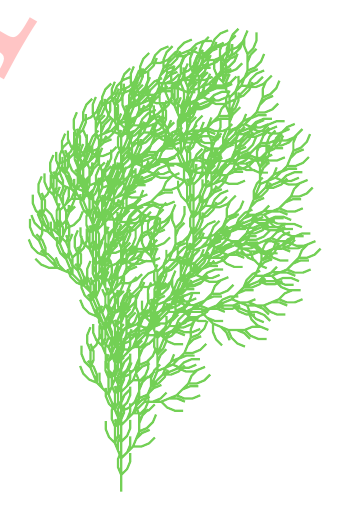
\begin{tikzpicture}
  \draw [GREEN, thick, rotate=90]
    [l-system={rule set={F -> FF-[-F+F+F]+[+F-F-F]}, axiom=F, order=4, step=3pt, angle=22.5}]
    lindenmayer system;
\end{tikzpicture}
\end{center}

\end{document}